\PassOptionsToPackage{table}{xcolor}
\documentclass[pdf]{beamer}
\mode<presentation>{\usetheme{Dresden}}
\usepackage{lmodern}
\usepackage[normalem]{ulem}
\usepackage{amsmath,textcomp,amssymb,geometry,graphicx,listings,array,color,amsthm}

\usepackage[noend]{algpseudocode}

\usepackage[
backend=biber,
sorting=ynt,
]{biblatex}
\addbibresource{lecture.bib}

\usepackage{tikz}
\usepackage{multicol}
\usetikzlibrary{shapes,snakes}
\usetikzlibrary{positioning}
\usetikzlibrary{arrows}
\usetikzlibrary{fit}
\usetikzlibrary{math}

%% For on-slide alerting of nodes
\tikzstyle{alert} = [text=black, fill=blue!20, draw=black]
\setbeamercolor{alerted text}{fg=blue}
\tikzset{alerton/.code args={<#1>}{%
  \only<#1>{\pgfkeysalso{alert}} % \pgfkeysalso doesn't change the path
}}

%% utils for removing uninteresting sections from the navbar
%% https://tex.stackexchange.com/questions/317774/hide-section-from-sidebar
\makeatletter
\let\beamer@writeslidentry@miniframeson=\beamer@writeslidentry%
\def\beamer@writeslidentry@miniframesoff{%
  \expandafter\beamer@ifempty\expandafter{\beamer@framestartpage}{}% does not happen normally
  {%else
    % removed \addtocontents commands
    \clearpage\beamer@notesactions%
  }
}
\newcommand*{\miniframeson}{\let\beamer@writeslidentry=\beamer@writeslidentry@miniframeson}
\newcommand*{\miniframesoff}{\let\beamer@writeslidentry=\beamer@writeslidentry@miniframesoff}
\makeatother

%% preamble
\title{NASA CARA}
\subtitle{Air Traffic Control \emph{in Spaaaaaaaaace}}
\author{A.C.}
\date{\today}

\AtBeginSection[]
{
  \miniframesoff
  \begin{frame}{Outline}
    \tableofcontents[currentsection,hideothersubsections]
  \end{frame}
  \miniframeson
}

\definecolor{darkred}{rgb}{0.7,0,0}
\definecolor{darkgreen}{rgb}{0,0.5,0}
\definecolor{darkblue}{rgb}{0,0,0.5}
\definecolor{darkpurple}{rgb}{0.4, 0.0, 0.4}

%% Code font settings
\lstset{
  showstringspaces=false,
  basicstyle=\scriptsize\ttfamily,
  commentstyle=\color{darkred},
  stringstyle=\color{darkgreen},
  keywordstyle=\bfseries\color{darkpurple},
}

%%%%%%%%%%%%%%%%%%%%%%%%%%
% Start of Actual slides %
%%%%%%%%%%%%%%%%%%%%%%%%%%
\begin{document}
\begin{frame}
  \titlepage
\end{frame}

\section{CARA Mission}
\subsection{Purpose}
\begin{frame}{CARA in Theory}
  Mission Statement:
  \begin{quote}
    To take prudent measures, at reasonable cost, to enhance safety of flight,
    without placing an undue burden on mission operations
  \end{quote}
\end{frame}

\begin{frame}{CARA in Practice}
  Inputs:
  \begin{itemize}
  \item Ephemeris data from cooperating missions.
  \item Catalog of tracked earth-orbiting objects from Combined Space Operations
    Center (CSpOC).
  \end{itemize}

  Outputs:
  \begin{itemize}
  \item Alerts to protected missions on high interest events (HIEs).
  \item Advisories for protected missions on risk mitigations for HIEs.
    \begin{itemize}
    \item Hopefully avoid more Kosmos-Iridium incidents.
    \end{itemize}
  \end{itemize}
\end{frame}

\subsection{Complexity}
\begin{frame}{Kepler Orbits}
  \[ \ddot{R} = \ddot{R}_\text{2B} = \frac{Gm_\text{other}}{||R||^3}R \]

  \begin{itemize}
  \item Solution known since Kepler and Newton.
    \begin{itemize}
    \item Must be a conic section.
    \item If closed, then ellipse.
    \end{itemize}
  \item A star holds its course and its aim\ldots returns and returns\ldots and is always the same
    \begin{itemize}
    \item \textit{Mais non}
    \end{itemize}
  \end{itemize}
\end{frame}

\begin{frame}{Perturbation: Third Bodies}
  \[ \ddot{R} = \ddot{R}_\text{2B} + \alert{\ddot{R}_\text{PM}}\]

  \begin{itemize}
  \item Gravity is a universal force.
  \item Lots of non-earth mass out there
    \begin{itemize}
    \item Luna
    \item Sol
    \item Uncounted others (fortunately negligible)
    \end{itemize}
  \item Particularly relevant for higher-altitude orbits.
  \item Additional bodies also accelerate Earth.
    \begin{itemize}
    \item Must subtract out ``shaky camera'' effect on our reference body.
    \end{itemize}
  \end{itemize}
\end{frame}

\begin{frame}{Perturbation: Non-Sphericity}
  \[ \ddot{R} = \ddot{R}_\text{2B} + \ddot{R}_\text{PM} + \alert{\ddot{R}_\text{NS}} \]
  \begin{itemize}
  \item $\ddot{R}_\text{2B}$ uses point-mass equations
    \begin{itemize}
    \item Works for points
    \item Works for spheres (shell theorem)
    \end{itemize}
  \item Earth is neither
    \begin{itemize}
    \item Tidal forces (order meters)
    \item Centrifugal forces (order kilometers)
    \end{itemize}
  \end{itemize}
\end{frame}

\begin{frame}[fragile]{Non-Sphericity: Oblation}
  Gross exaggeration: cylindrical Earth
  
  \begin{center}
    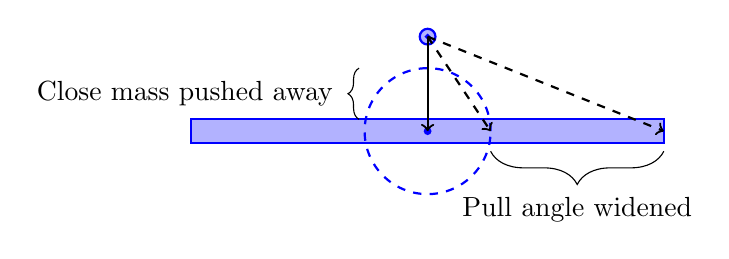
\begin{tikzpicture}
      \tikzmath{
        \h = 0.3;
        \w = 6;
        \rDot = 0.02;
        \rSat = 0.1;
        \r = 0.8;
      }

      \coordinate (C) at (\w / 2, \h / 2);
      \coordinate (P) at (\w / 2, \h /2 + 1.5*\r);
      
      \draw[blue, thick, fill=blue, fill opacity=0.30] rectangle (\w,\h);
      \draw[blue, thick, dashed] (C) circle [x radius = \r, y radius = \r];


      \filldraw[blue, thick, fill=blue, fill opacity=0.30] (P) circle [x radius = \rSat, y radius = \rSat];
      \filldraw[blue, thick] (P) circle [x radius = \rDot, y radius = \rDot]; 

      \node[circle,fill=blue,inner sep=1pt,minimum size=\rDot] (CN) at (C) {};
      
      \draw[black,thick,->] (P) -- (C);
      \draw [decorate,decoration={brace,amplitude=4pt,mirror,raise=2pt}]
      (\w / 2 - \r, \h/2 + \r) -- (\w / 2 - \r, \h) node[midway,xshift=-8pt,left]{Close mass pushed away};


      
      \draw[black,thick, dashed, ->] (P) -- (\w /2 + \r, \h /2);
      \draw[black,thick, dashed, ->] (P) -- (\w, \h /2);

      
      \draw [decorate,decoration={brace,amplitude=12pt,mirror,raise=3pt}]
      (\w / 2 + \r, 0) -- (\w, 0) node[midway,yshift=-16pt,below]{Pull angle widened};

    \end{tikzpicture}
  \end{center}

  Polar gravity $\downarrow\downarrow\downarrow$.
\end{frame}

\begin{frame}{Perturbation: Indirect Oblation}
  \[ \ddot{R} = \ddot{R}_\text{2B} + \ddot{R}_\text{PM} + \ddot{R}_\text{NS}  + \alert{\ddot{R}_\text{IO}}\]
  \begin{itemize}
  \item Earth is (still) not an inertial reference frame.
  \item Point-mass effects already smoothed out in $\ddot{R}_\text{PM}$ term.
  \item Non-sphericity effects can further perturb our reference frame.
    \begin{itemize}
    \item Almost always negligible.
    \item Earth-Luna interaction is measurable, however.
    \end{itemize}
  \end{itemize}
\end{frame}

\begin{frame}{Perturbation: Drag}
  \[ \ddot{R} = \ddot{R}_\text{2B} + \ddot{R}_\text{PM} + \ddot{R}_\text{NS}  + \ddot{R}_\text{IO} + \alert{\ddot{R}_\text{D}} \]

  \begin{itemize}
  \item Drag equation: $F_\text{D} = \frac{1}{2}\rho v^2 C_\text{D} A$
  \item Scales by
    \begin{itemize}
    \item Object shape and orientation ($C_\text{D}, A$).
    \item Square of object velocity $v^2$.
    \item Atmospheric density $\rho$, drops exponentially with altitude.
    \end{itemize}
  \item LEO objects (altitude $< 2000$ km) are low and fast
    \begin{itemize}
    \item experience non-negligible drag
    \end{itemize}
  \item Bonus: non-periodic and non-conservative.
  \end{itemize}
\end{frame}

\begin{frame}{Perturbation: Solar Radiation Pressure}
  \[ \ddot{R} = \ddot{R}_\text{2B} + \ddot{R}_\text{PM} + \ddot{R}_\text{NS}  + \ddot{R}_\text{IO} + \ddot{R}_\text{D} + \alert{\ddot{R}_\text{SRP}}\]

  \begin{itemize}
  \item $\gamma := \sqrt{\frac{c^2}{c^2 - v^2}}$
  \item $ p = \gamma m v$
  \item photons: $m\rightarrow0, \gamma \rightarrow \infty $
    \begin{itemize}
    \item $p \rightarrow ?$
    \item God's math: $ p = \frac{h}{\lambda} $
    \end{itemize}
  \item Absorbing and emitting light imparts momentum
    \begin{itemize}
    \item Sunlight never stops: SRP
    \item Most impactful on higher altitude orbits
    \item Non-periodic and non-conservative
    \end{itemize}
  \end{itemize}
\end{frame}

\begin{frame}{Perturbation: Thrust}
  \[ \ddot{R} = \ddot{R}_\text{2B} + \ddot{R}_\text{PM} + \ddot{R}_\text{NS}  + \ddot{R}_\text{IO} + \ddot{R}_\text{D} + \ddot{R}_\text{SRP} + \alert{\ddot{R}_\text{T}} \]

  \begin{itemize}
  \item Orbital payloads commonly come equipped with maneuvering thrusters
    \begin{itemize}
    \item Chemical burns (fast, short)
    \item Electric propulsion (slow, long)
    \end{itemize}
  \item Good news: allows for doing something about predicted collisions
  \item Bad news: Non-periodic, non-conservative, AND non-physical(-ish)
  \end{itemize}
\end{frame}

\begin{frame}{Perturbation Impacts}
  \begin{itemize}
  \item Low-to-medium fidelity diff-eqs can be solved analytically
    \begin{itemize}
    \item E.g. Brouwer models, SGP4/SDP4
    \end{itemize}
  \item High-fidelity generally resort to numerical integration
    \begin{itemize}
      \item E.g. NORAD Special Perturbations (SP)
    \end{itemize}
  \item Low- and high-fidelity models can diverge significantly, rapidly
    \begin{itemize}
    \item By kilometers
    \item Within a few orbital periods (i.e. hours)
    \end{itemize}
  \item None of the models correspond to beautiful, eternal shapes.
  \end{itemize}
\end{frame}

\subsection{Consequence}

\begin{frame}{Mission Safety}
  \[ E(\text{Cost}(X)) = P(X) \cdot \text{Cost}(X) \]
  
  \begin{itemize}
  \item Plausible $\text{Cost}(X)$: 100 million USD
  \item Plausible $P(X)$: 2e-4
  \item $E(\text{Cost}(X)) = 2 \cdot 10^{-4} \cdot 10^8 = 20000$ USD
    \begin{itemize}
    \item Might be worth mitigating
    \item Although, $\sim 85\%$ of likely-lethal conjunctors aren't even
      tracked \ldots
    \end{itemize}
  \end{itemize}
\end{frame}

\begin{frame}{Domain Safety}

  \begin{itemize}
  \item Any collision increases hazard to ecosystem
    \begin{itemize}
    \item Debris potential strongly linked to object size
    \item Largest objects are best tracked
    \item Objects follow a power-law distribution: many, many small pieces,
      comparatively few large
    \end{itemize}
    \pause

  \item Orbit contention is self-reinforcing
    \begin{itemize}
    \item More objects means more conjunctions
    \item More conjunctions means more collisions
    \item More collisions means more objects
    \end{itemize}
    \pause
  \item Critical density $\rightarrow$ runaway, sustained fragmentation
    \begin{itemize}
    \item Kessler syndrome
    \end{itemize}
  \end{itemize}
\end{frame}

% \begin{frame}{Domain Safety II}
%   \begin{itemize}
%   \item Vested public interest in controlling flux
%   \item Must avoid collisions, especially between large objects
%   \end{itemize}
% \end{frame}

\section{Conjunction Identification}
\subsection{Volumetric Screening}

\begin{frame}{Conjunction Screening}
  \begin{itemize}
  \item Before a conjunction can be analyzed it must be identified
    \begin{itemize}
    \item Want to know the time of closest approach (TCA)
    \item and of course the conjunctors' states at TCA
    \end{itemize}
  \item Technically not a CARA responsibility
    \begin{itemize}
    \item Screening computed for CARA by CSpOC using COMBO (Computation of Miss
      Between Orbits).
    \item Operates on a ``flying-ellipsoid'' volumetric screening paradigm.
    \end{itemize}
  \end{itemize}
\end{frame}

\begin{frame}[fragile]{Volumetric Screening}
  \begin{center}
    \begin{tikzpicture}
      \tikzmath{
        \rDot = 0.04;
      }

      \coordinate (P1) at (50:4 and 5);
      \coordinate (P2) at (40:4 and 5);
      \coordinate (P3) at (30:4 and 5);
      \draw[black, thick, dashed] (0:4 and 5) arc (0:90:4 and 5);
      
      \coordinate (S1) at (80:6 and 4);
      \coordinate (S2) at (70:6 and 4);
      \coordinate (S3) at (60:6 and 4);
      \draw[black, thick, dashed] (0:6 and 4) arc (0:90:6 and 4);

      \node (PLabel) at (1,2) {Primary};
      \node (SLabel) at (4,5) {Secondary};

      % I'm fairly certain this can be cleaned up with a for-loop, but my
      % tikz-fu is still kind of weak and copy-paste is easy.
      \only<1>{
        \node[circle,fill=blue,inner sep=1pt,minimum size=\rDot] (P1N) at (P1) {};
        \node[circle,fill=red,inner sep=1pt,minimum size=\rDot] (S1N) at (S1) {};
        \draw[black, ->] (PLabel) -- (P1N);
        \draw[black, ->] (SLabel) -- (S1N);

        \draw[blue, rotate=50, fill=blue, fill opacity=.30] (P1) circle (0.5 and 2);
        \draw[blue, rotate=50, shift=(P1)] (0, 2) arc (90:270:0.25 and 2);
        \draw[blue, dashed, rotate=50, shift=(P1)] (0, -2) arc (-90:90:0.25 and 2);
      }
      \only<2>{
        \node[circle,fill=blue,inner sep=1pt,minimum size=\rDot] (P2N) at (P2) {};
        \node[circle,fill=red,inner sep=1pt,minimum size=\rDot] (S2N) at (S2) {};
        \draw[black, ->] (PLabel) -- (P2N);
        \draw[black, ->] (SLabel) -- (S2N);

        \draw[blue, rotate=40, fill=blue, fill opacity=.30] (P2) circle (0.5 and 2);
        \draw[blue, rotate=40, shift=(P2)] (0, 2) arc (90:270:0.25 and 2);
        \draw[blue, dashed, rotate=40, shift=(P2)] (0, -2) arc (-90:90:0.25 and 2);
      }
      \only<3>{
        \node[circle,fill=blue,inner sep=1pt,minimum size=\rDot] (P3N) at (P3) {};
        \node[circle,fill=red,inner sep=1pt,minimum size=\rDot] (S3N) at (S3) {};
        \draw[black, ->] (PLabel) -- (P3N);
        \draw[black, ->] (SLabel) -- (S3N);

        \draw[blue, rotate=30, fill=blue, fill opacity=.30] (P3) circle (0.5 and 2);
        \draw[blue, rotate=30, shift=(P3)] (0, 2) arc (90:270:0.25 and 2);
        \draw[blue, dashed, rotate=30, shift=(P3)] (0, -2) arc (-90:90:0.25 and 2);
      }

      
    \end{tikzpicture}
  \end{center}
\end{frame}

\begin{frame}{Volumetric Screening}
  \begin{algorithmic}
    \Procedure{ScreenConjunctions}{}
    \For{$p, s, t \in \textit{Primaries} \times \textit{Secondaries} \times \textit{Time Slices}$}
      \State $V \gets \text{ellipse around }p(t)$
      \If{$s(t).\text{pos} \notin V$}
        \State \textbf{continue}
      \EndIf
      \State $d(\tau) := || p(\tau).\text{pos}  - s(\tau).\text{pos} ||$
      \If{$\text{sign}(d'(t)) = \text{sign}(d'(t+\Delta t))$}
        \State \textbf{continue}
      \EndIf
      \State $t^* \gets \operatorname*{argmin}_{[t, t + \Delta t]} d$
      \State $\text{Emit } (p, s, t^*)$
    \EndFor
    \EndProcedure  
  \end{algorithmic}
\end{frame}

\section{HIE Identification}
\subsection{Risk Measures}

\begin{frame}{Standoff Distance}
  \begin{itemize}
  \item Most intuitive measure of safety
    \begin{itemize}
    \item If we are far apart, of course we aren't touching.
    \item Implicitly part of volumetric screening regimes.
    \end{itemize}

  \item Difficult to map distance onto risk.
    \begin{itemize}
    \item How far apart is far? Meters? Kilometers?
    \end{itemize}
    
  \item Cannot capture uncertainty
    \begin{itemize}
    \item What if our measurements of a satellite's state are known to be imprecise?
    \end{itemize}
    
  \item Tendency toward conservatism
    \begin{itemize}
      \item sometimes desirable, e.g. around human space flight assets
    \end{itemize}
  \end{itemize}
\end{frame}

\begin{frame}{Probability of Collision}
  \begin{itemize}
  \item Most commonly used measure of safety.

  \item Answers the challenges with standoff distance
    \begin{itemize}
    \item Maps naturally to risk.
    \item Captures and describes uncertainty and imprecision.
    \item Allows for mindfully tuned risk postures.
    \end{itemize}

  \item But! Can suffer from probability dilution.
    \begin{itemize}
    \item Space is big. Really big. Really, really big.
    \item Rubbish measurements $\Rightarrow P_C \approx 0$.
    \item Probability is ``diluted'' across space.
    \end{itemize}
  \end{itemize}
\end{frame}

\subsection{2D $P_C$}
\begin{frame}{Naive $P_C$}

  \[ \int\int \rho(S_1,S_2) \mathbb{I}(\text{collision} | S_1,S_2) dS_1 dS_2 \]

  \begin{itemize}
  \item That's a 12-dimensional integral.
  \item $\mathbb{I}(\text{collision} | S_1,S_2)$ is a nightmare function.
  \item Let's make some simplifying assumptions
  \end{itemize}
\end{frame}

\begin{frame}{2D $P_C$: Assumptions}
  \begin{enumerate}
  \item State position vectors $R_1 \sim \mathcal{N}(\bar{R_1}, C_1), R_2 \sim \mathcal{N}(\bar{R_2}, C_2)$
  \item $R_1 \perp R_2$
  \item Velocity uncertainty is negligible
  \item Position uncertainty is stable throughout the encounter
  \item Relative motion is linear throughout the encounter
  \item Both objects are spheres
  \end{enumerate}
\end{frame}

\begin{frame}{2D $P_C$}
  Core idea: Don't think about two objects, think about
  the distance separating them. More precisely, let
  
  \[ R_\text{miss} := R_2 - R_1 \]

  We wish to integrate

  \[ \int \rho_\text{miss}(R) \mathbb{I}(\text{collision} | R) dR \]
\end{frame}

\begin{frame}{2D $P_C$}

  \[ \int \alert{\rho_\text{miss}(R)} \mathbb{I}(\text{collision} | R) dR \]

  Recall: $R_1 \perp R_2$, both Gaussian. So

  \[ R_\text{miss} \sim \mathcal{N}(\bar{R_2} - \bar{R_1}, C_2 - C_1) \]

  $\rho_\text{miss}$ is just $\phi$!
\end{frame}


\begin{frame}{2D $P_C$}

  \[ \int \rho_\text{miss}(R) \alert{\mathbb{I}(\text{collision} | R)} dR \]

  Linear motion, spherical objects. Collision iff $\exists t \in \mathbb{R}$ s.t.

  \[ ||R_\text{miss} + v_\text{miss} \cdot t|| < \text{HBR}_1 + \text{HBR}_2 \]

  That's a cylinder!

  \begin{center}
    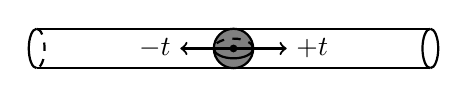
\begin{tikzpicture}
      \tikzmath{
        \h = 0.5;
        \w = 5;
        \r = \h / 2;
        \rDot = 0.02;
      }

      % \fill[fill=gray] (0, 0) rectangle (\w, \h);
      % cylinder
      \draw[black, thick] (0, 0) -- (\w, 0);
      \draw[black, thick] (0, \h) -- (\w, \h);
      \draw[black, thick] (0,0) arc (270:90:0.1 and \h / 2);
      \draw[black, thick, dashed] (0,\h) arc (90:-90:0.1 and \h / 2);
      \draw[black, thick] (\w,0) arc (270:90:0.1 and \h / 2);
      \draw[black, thick] (\w,\h) arc (90:-90:0.1 and \h / 2);
      % sphere
      \coordinate (C) at (\w / 2, \h /2);
      \draw[black, thick, fill=gray] (C) circle [x radius = \r, y radius = \r];
      \draw[black, thick, shift=(C)] (-\r,0) arc (180:360:\r + 0 and \r / 2);
      \draw[black, thick, dashed,shift=(C)] (\r,0) arc (0:180:\r + 0 and \r / 2);

      \node (TPlus) at (1 + \w / 2, \h / 2 ) {$+t$};
      \node (TMinus) at (-1 + \w / 2, \h / 2 ) {$-t$};

      \draw[black, thick, ->] (C) -- (TPlus);
      \draw[black, thick, ->] (C) -- (TMinus);
      \node[circle,fill=black,inner sep=1pt,minimum size=\rDot] (CDot) at (C) {};
    \end{tikzpicture}
  \end{center}
\end{frame}


\begin{frame}{2D $P_C$}
  Rotate coordinates to align cylinder with $z$-axis.

  \begin{center}
    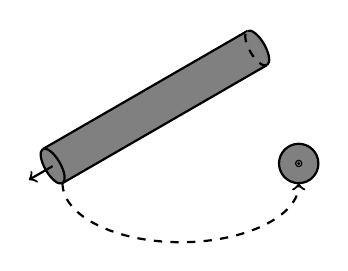
\begin{tikzpicture}
      \tikzmath{
        \h = 0.5;
        \w = 3;
        \r = \h / 2;
        \rDot = 0.02;
      }
      % cylinder
      \fill[fill=gray,rotate=30] (0, 0) rectangle (\w, \h);
      \draw[black, thick,fill=gray,rotate=30] (0, 0) -- (\w, 0);
      \draw[black, thick,fill=gray,rotate=30] (0, \h) -- (\w, \h);
      \draw[black, thick,fill=gray,rotate=30] (0,0) arc (270:90:0.1 and \h / 2);
      \draw[black, thick,fill=gray,rotate=30] (0,\h) arc (90:-90:0.1 and \h / 2);
      \draw[black, thick,fill=gray,rotate=30,dashed] (\w,0) arc (270:90:0.1 and \h / 2);
      \draw[black, thick,fill=gray,rotate=30] (\w,\h) arc (90:-90:0.1 and \h / 2);
      \draw[black, thick,rotate=30, ->] (0,\h / 2) -- (-0.35, \h / 2);

      % circle
      \coordinate (C) at (3, 0.25);
      \draw[black, thick, fill=gray] (C) circle [radius = \h / 2];
      \fill[fill=black] (C) circle [radius = \rDot];
      \draw[black] (C) circle [radius = \rDot * 2];

      % Rotation arrow
      \draw[black, thick, dashed, ->] (0, 0) arc (180:360:1.5 and 0.75);

    \end{tikzpicture}
  \end{center}
  
  Cylinder is infinite: $z$-axis marginalizes to 1.
\end{frame}

\begin{frame}{2D $P_C$}

  Integral form after massaging:
  
  \[ P_C = \frac{1}{\sqrt{\det(2\pi C)}} \int\int_A \exp \left( -\frac{r^TC^{-1}r}{2}\right)dxdy \]

  Not fully analytic, but quite amenable to numerical quadrature.

\end{frame}

\subsection{3D $P_C$}

\begin{frame}{Hyperkinetic Assumptions}
  \begin{itemize}
  \item 2D $P_C$ treated conjunctors like a pair of bullets
  \item Pretty good model when relative velocity is high, encounter is short
  \item Not all close approaches occur at high (relative) velocity, though
  \item Can we do better?
  \end{itemize}
\end{frame}

\begin{frame}{3D $P_C$}
  What happens if we try to count collisions throughout the encounter?

  \[ \bar{N}_C = \int_{t_0}^{t_\text{end}} E(\dot{N}_C) dt\]

  That's not actually $P_C$, but for single-encounter conjunctions, the
  distinction is academic.
\end{frame}


\begin{frame}{3D $P_C$}
  \[ E(\dot{N}_C) = \int \int \rho(S_1, S_2) \alert{\dot{N}_C(S_1, S_2, t)} dS_1dS_2\]

  To find $\dot{N}_C(S_1, S_2, t)$, let's start with $N_\text{overlap}$. It's a step function on the
  ball around our miss vector, propagated to time $t$!

  \[ N_\text{overlap} = \mathbb{I}(||R_\text{miss}|| < r) = H(r^2 - R^T R) \]

  Chain rule it out to get

  \[ \dot{N}_\text{overlap} = \delta(r^2 - R^T R)(-2R^T \dot{R})\]
\end{frame}

\begin{frame}{3D $P_C$}

  \[ E(\dot{N}_C) = \int \int \rho(S_1, S_2) \alert{\dot{N}_C(S_1, S_2, t)} dS_1dS_2\]

  $\dot{N}_\text{overlap}$ is not $\dot{N_\text{C}}$ -- it adds ingress
  (yay!) and subtracts egress (boo!). Thresholding at zero solves our problem

  \[ \dot{N}_C = max(0, \dot{N}_\text{overlap}) = \delta(r^2 - R^T R)[-2R^T \dot{R}]_{+}\]
  
\end{frame}

\begin{frame}{3D $P_C$}

  \[ E(\dot{N}_C) = \alert{\int \int \rho(S_1, S_2)} \dot{N}_C(S_1, S_2, t) \alert{dS_1dS_2}\]

  \begin{itemize}
  \item Hello \sout{darkness} 12-D integral, my old friend
  \item With an assumption of elliptical movement, this \emph{can} actually be
    reduced to a manageable dimension.
    \begin{itemize}
    \item Requires a heroic amount of massaging algebra and calculus.
    \item Interested parties are referred to the full pub.
    \end{itemize}
  \item Final integral dimensions post-massage:
    \begin{itemize}
    \item  1-D time integral over the encounter interval
    \item  2-D surface integral over the miss ball
    \end{itemize}
  \end{itemize}
\end{frame}



\subsection{Monte Carlo}

\begin{frame}{Motivation}
  \begin{itemize}
  \item All this integration, it's making my head hurt.
  \item Even the fancy 3D $P_C$ variant had to make simplifying assumptions.
  \item This is a stochastic process, let's try modeling it stochastically.
  \end{itemize}
\end{frame}

\begin{frame}{From-Epoch MC}
  \begin{algorithmic}
    \Procedure{FromEpochMC}{\textit{primOD}, \textit{secOD}, \textit{trials}}
    \State $\textit{hits} \gets 0$
    \For{$i \in [0,\ldots,\textit{trials})$}
      \State $p \gets \text{draw from } \textit{primOD}$ 
      \State $s \gets \text{draw from } \textit{secOD}$
      \If{$p.\text{propagate()} \text{ collides with } s.\text{propagate()}$}
        \State $\textit{hits} \gets \textit{hits} + 1$
      \EndIf
      \EndFor
    \State \Return $\frac{\textit{hits}}{\textit{trials}}$
    \EndProcedure  
  \end{algorithmic}
\end{frame}

\begin{frame}{From-Epoch MC}
  \begin{itemize}
  \item No simplifying assumptions! Estimate is as good as
    \begin{itemize}
    \item Our orbit propagation algorithm
    \item The number of trials we run
    \end{itemize}
  \item Heinously expensive, though
    \begin{itemize}
    \item Millions and millions of trials
    \item Each trial doing high-fidelity numerical ODE solving from epoch up
      through TCA
    \end{itemize}
  \item Most useful to prove out the accuracy of other algorithms.
  \end{itemize}
\end{frame}

\begin{frame}{From-TCA MC}
  \begin{algorithmic}
    \Procedure{FromTCAMC}{\textit{primTCA}, \textit{secTCA}, \textit{trials}}
    \State $\textit{hits} \gets 0$
    \For{$i \in [0,\ldots,\textit{trials})$}
      \State $p \gets \text{draw from } \textit{primTCA}$ 
      \State $s \gets \text{draw from } \textit{secTCA}$
      \If{$p.\text{propForward()} \text{ collides with } s.\text{propForward()}$}
        \State $\textit{hits} \gets \textit{hits} + 1$
      \ElsIf{$p.\text{propBack()} \text{ collides with } s.\text{propBack()}$}
        \State $\textit{hits} \gets \textit{hits} + 1$
      \EndIf
      \EndFor
    \State \Return $\frac{\textit{hits}}{\textit{trials}}$
    \EndProcedure  
  \end{algorithmic}
\end{frame}

\begin{frame}{From-TCA MC}
  \begin{itemize}
  \item Faster than From-Epoch
    \begin{itemize}
    \item Only need to propagate motion around the encounter
    \item Shorter motion-prop window means lower fidelity propagation schemes
      can be used.
    \end{itemize}
  \item Depends on assumptions about the shape of propagated uncertainty
    \begin{itemize}
    \item Not really a practical issue if we're careful to sample in curvilinear
      coordinates.
    \end{itemize}
  \item Still much slower than analytic methods.
    \begin{itemize}
    \item Empirically not much better results
    \item Not frequently used in CARA in practice
    \end{itemize}
  \end{itemize}
\end{frame}

\section{Risk Remediation}
\subsection{Maneuver Planning}

\begin{frame}{HIE Response}

  Two choices for dealing with an HIE.
  
  \begin{enumerate}
  \item Change course
    \begin{itemize}
    \item Costs fuel/reaction mass.
    \item Generally cheaper the earlier an orbit is modified.
    \end{itemize}
  \item Wait and see
    \begin{itemize}
    \item Most HIEs come to nothing
    \item Can self-resolve ``early enough'' as conjunction nears and uncertainty
      drops off.
    \end{itemize}
  \end{enumerate}

  Common pattern: plan maneuver immediately in response to HIE, then abort if
HIE resolves before the commit point.
\end{frame}

\begin{frame}{Maneuver Trade Space}
  \begin{itemize}
  \item Several knobs to turn when modifying trajectory
    \begin{itemize}
    \item Burn intensity
    \item Burn timing
    \item Satellite orientation (differential drag)
    \end{itemize}
  \item CARA maintains analysis tools for mapping possible maneuvers to expected
    $P_C$ post-maneuver.
    \begin{itemize}
    \item Not very well documented in the public domain\ldots
    \end{itemize}
  \item Allows us to mitigate the risk to the primary from this particular
    secondary.
  \item What about all the other possible conjunctors?
  \end{itemize}
\end{frame}

\begin{frame}{Maneuver Validation}
  \begin{itemize}
  \item Space is big.
  \item The lane we plan to swerve into is \emph{probably} open.
  \item Approach: Plan the remediation in isolation, then pass the planned orbit back into the next round of conjunction screening.
    \begin{itemize}
    \item If no new HIEs crop up, we're good.
    \item Else, try planning a different maneuver.
    \end{itemize}
  \end{itemize}
\end{frame}

%% Q&A and Further reading.
\miniframesoff
\section*{}
\begin{frame}{References and Further Reading}
  \AtNextBibliography{\tiny}
  \nocite{*}
  \printbibliography
\end{frame}

\begin{frame}{Self Link}
  The source for this presentation is hosted at
\url{https://github.com/alan-christopher/cara-edu}.

\end{frame}
\end{document}
